\documentclass[../../thesis.tex]{subfiles}

\begin{document}

Our work in this thesis can be seen as a tangent of the paper "Vector Quantized Time Series Generation with a Bidirectional Prior Model" \cite{TimeVQVAE}. 
We simplify the model architecture by omitting the high-low frequency split, which reduces the model to what they refer to as "naive TimeVQVAE" in their paper. We expand on naive TimeVQVAE  with a self-supervised extension.\newline

A schematic figure of our proposed tokenization model is given in \ref{fig:NC-VQVAE}. To improve on the reconstruction we add a regularizing term by reconstructing augmented views. We hypothesize that the model generalizes better to unseen data by letting the decoder "see" the augmented views.\newline
To separate classes better we introduce a non contrastive self supervised loss. The intuition being that the representation of original and augmented views are pushed closer together by the SSL loss. We further enforce this hypothesis by using augmentations that preserve the overall semantics of the class conditional distributions. \newline

\section{Proposed model: NC-VQVAE}

Our model, termed NC-VQVAE, is a generative time series model which learns expressive discrete latent representations by combining VQVAE \cite{VQVAE} with non contrastive self supervised learning algorithms. NC-VQVAE uses the two staged modelling approach presented in \cite{TimeVQVAE}, and can be considered an extension of their "naive TimeVQVAE". Our model mainly extends the tokenization stage, where we incorporate Barlow Twins \cite{zbontar2021barlow} and VIbCReg \cite{lee2024computer} as our non contrastive SSL, but the framework is flexible. For stage two we model the prior using a bidirectional transformer as MaskGIT \cite{chang2022maskgit}.

\subsection{NC-VQVAE}

The architecture of the tokenization model \ref{fig:NC-VQVAE} consists of two branches. The top and bottom branch is referred to as the original and augmented branch respectively. The model takes a time series $x$ as input and creates an augmented view $x'$. The original branch is simply the naive TimeVQVAE from \cite{TimeVQVAE}, while the augmented branch is an autoencoder, constructed by omitting the quantization layer. The views are passed through their respective branches, where we compute the SSL loss derived from the original discrete latent representation $z_q$ and the augmented continuous latent $z'$, before the decoder reconstructs each latent representation. \newline 
The SSL loss is calculated by concatenate the average and max pool of both representations individually and pass the resulting vectors to the projector. \newline

\begin{figure}[h]
    \label{fig:NC-VQVAE}
    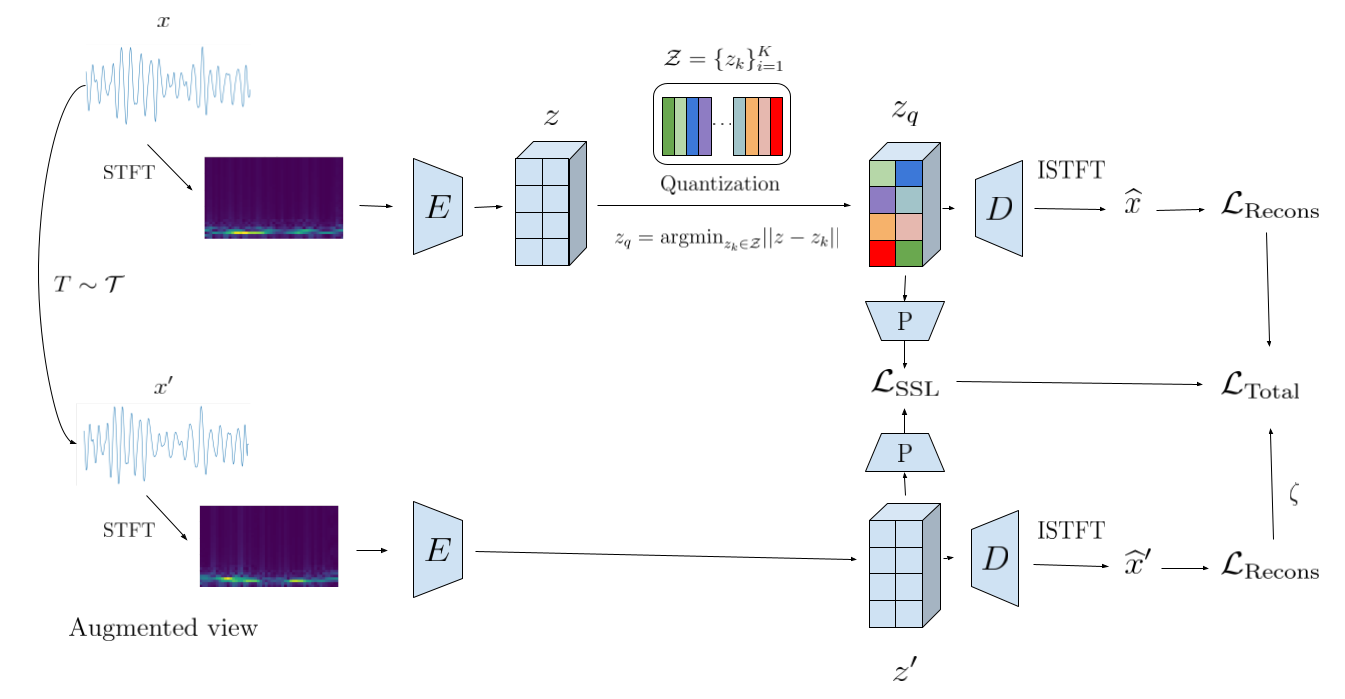
\includegraphics[scale=0.27]{Siam-VQVAE.png}
    \centering  
    \caption{Overview of proposed model. NC-VQVAE}
\end{figure}

For prior learning we follow MaskGIT and refer to related works for a description of the learning and generation procedure.

% \subsubsection{Non contrastive SSL}
% We calculate the SSL loss using the discrete latent representation $z_q$ and the augmented continuous latent $z'$. We concatenate the average and max pool of both representations individually and pass the resulting vectors to the projector. 

% \subsubsection{Loss}
% VQVAE, SSL: VIbCReg and BarlowTwins, AugRecons



% \subsubsection{Loss}

% \subsubsection{Implementation}


\end{document}